\section{Spezifische Anforderungen}
\subsection{Strukturierte Analyse}
\subsubsection{Kontextdiagramm}
\begin{figure}[H]
	\centering
  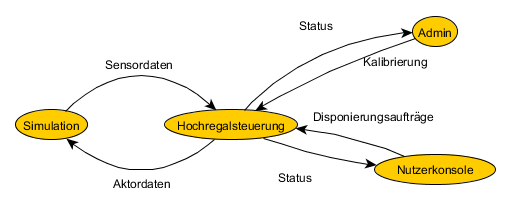
\includegraphics[width=\textwidth]{DFD/kontextdiagramm.png}
	\caption{Kontextdiagramm}
	\label{fig1}
\end{figure}
Aus dem Kontextdiagramm lässt sich leicht erkennen, dass das System aus zwei großen Teilen besteht. Auf der einen Seite ist sdie HRL-Steuerung, welche Eingaben erfasst, kontrolliert und die gewünschte Reaktion darauf berechnet. Auf der anderen Seite steht die Simulation, die für die physikalischen Abläufe nötige Zeit und das auslösen der diversen Sensoren simuliert. Verbunden sind beide durch diverse MessageQueues und eine globale Variable, welche in den weiteren Datenflussdiagrammen erleutert werden.
\subsubsection{DFD1 Simulation}
\begin{figure}[H]
	\centering
  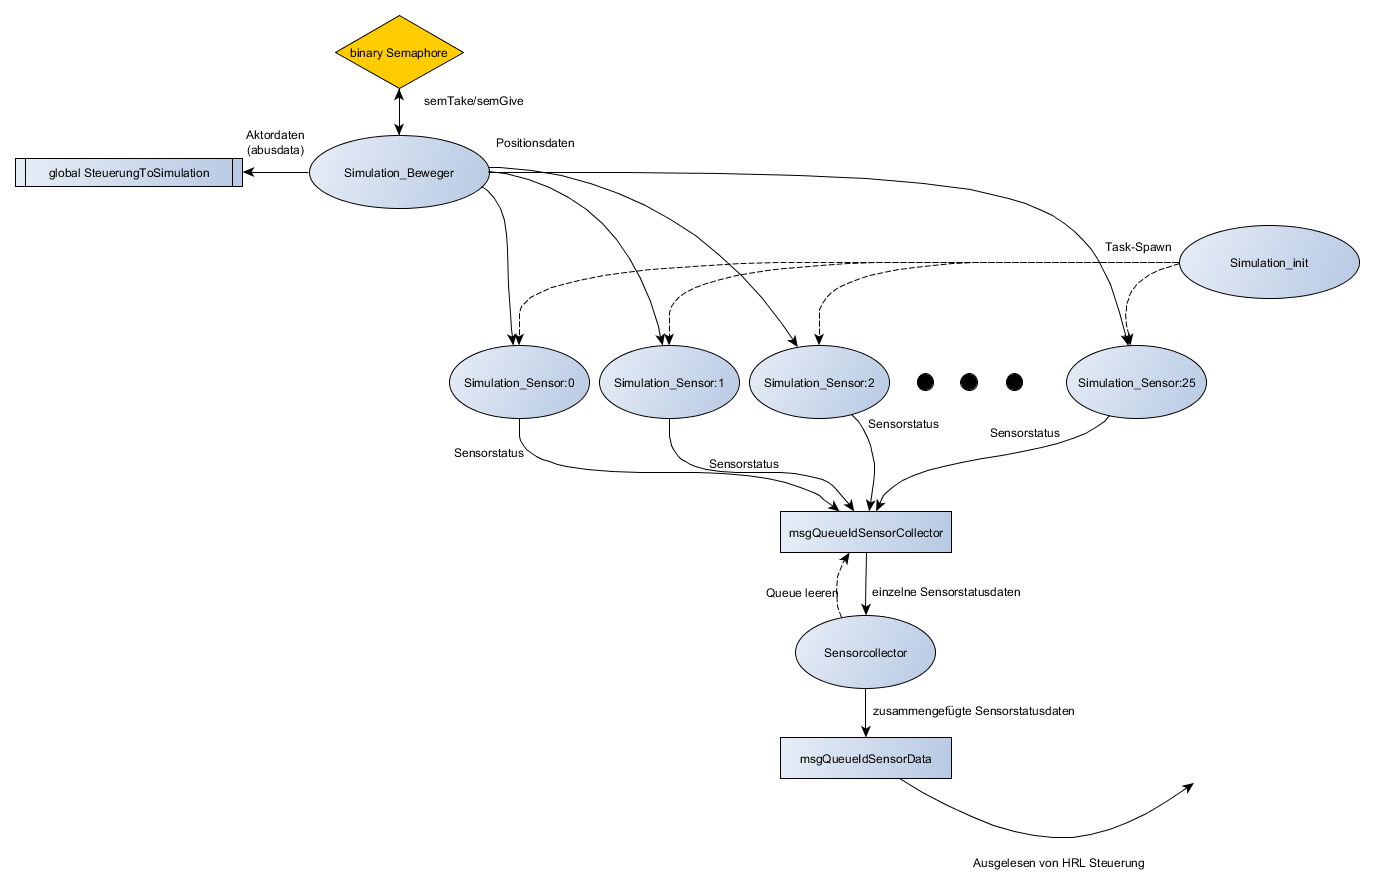
\includegraphics[width=\textwidth]{DFD/dfd1_simulation1_1.png}
	\caption{DFD1 Simulation}
	\label{fig2}
\end{figure}


\begin{figure}[H]
	\centering
  \includegraphics[width=\textwidth]{diagrams/gand.png}
	\caption{Gantt Diagramm der Task der Simulation}
	\label{gantt}
\end{figure}

Alle Tasks in der Simulation haben eine Priorität von 200 und ändern diese nicht. Sie werden in einer festen Reihenfolge erzeugt und laufen dann in jedem Zyklus in dieser Sequenz.\\
\\

\underline{Mini-Spec Simulation Beweger:}\\
Wie in Abb.\ref{gantt} zu sehen ist läuft der \textbf{Beweger} als erster Task eines Simulationsschrittes.
Der Beweger setzt virtuelle Position(Positionsdaten) nach Aktordaten (abusdata), welche durch einen Semaphore geschützt werden.  Da die Simulation minimal blockiert werden soll implementiert die Semaphore eine Prioritätsvererbung.\\ \\


\underline{Mini-Spec Simulation Sensor:}\\
Jeder Sensor bekommt eine ID die der bitstelle in Sensorbits entspricht. Zur initialisierung errechnet er so seine Position (\textit{triggeroffset}).\\ \\

\underline{Mini-Spec Simulation Sensor 0-22:}\\
Sensor Task berechnet eigenes \textit{triggeroffset} und gleicht dieses mit virtueller Position ab.\\
if(virtuelle Position-X == triggeroffset-X) true und eigene ID in \textit{msgQueueIdSensorCollector\\}
else false und eigene ID in \textit{msgQueueIdSensorCollector\\} \\
analog für Y- und Z-Sensoren\\ \\

\underline{Mini-Spec Simulation Sensor 23:}\\
Der Lichttaster wird gesetzt wenn er eine Auflade- bzw. Abladeoperation detektiert. Diese besteht (wie in Abb. \ref{fig3} zu sehen) aus unter den Ablagepunkt fahren, den Arm nach außen bzw. innen fahren und dann anheben, bzw. über den Ausgabepunkt fahren, den Arm nach außen bzw innen fahren und danach absenken.\\ \\

\underline{Mini-Spec Simulation Sensor 24-25:}\\
Sensoren für Lichtschranken.
Berechnung nicht über \textit{triggeroffset}, sondern die Lichtschranken werden über Zeitkonstanten gesteuert, welche hoch bzw. runter gezählt werden.\\
Setzen bzw. Entfernen eines Klötzchens aus bzw. in einen Lichttaster:\\ \\
if(Z = in Regal und Y= hoch) \\
Auslagerungsvorgang in Regal erkannt -> Lichttaster anschließend bedeckt und Belegungsmatrix[X][Y]= nicht belegt\\
\\
if(Z = in Regal und Y= runter)\\
Einlagerungsvorgang in Regal erkannt -> Lichttaster anschließend nicht bedeckt und Belegungsmatrix[X][Y] = belegt \\
\\
\\
if(Z = aus Regal heraus und Y= hoch)\\
Aufnahmevorgang in Eingabe-Slot erkannt -> Lichttaster anschließend bedeckt und Zeitkonstante von Lichtschrank in Slot wird zurückgesetzt\\
\\
if(Z = aus Regal heraus und Y= runter)\\
Auslagerungsvorgang in Ausgabe-Slot erkannt -> Lichttaster anschließend nicht bedeckt  Zeitkonstante von Lichtschrank in Slot wird zurückgesetzt\ \\
\\
\\
<<<<<<< Updated upstream
\underline{Mini-Spec Sensorcollector:}\\
Sensorcollector greift Datensatz aus msgQueueIdSensorCollector ab(leeren der Queue), fügt sie zu sbusdata zusammen und gibt diese in msgQueueIdSensorData\\ 


\subsubsection{DFD1 Steuerung}
\begin{figure}[H]
	\centering
  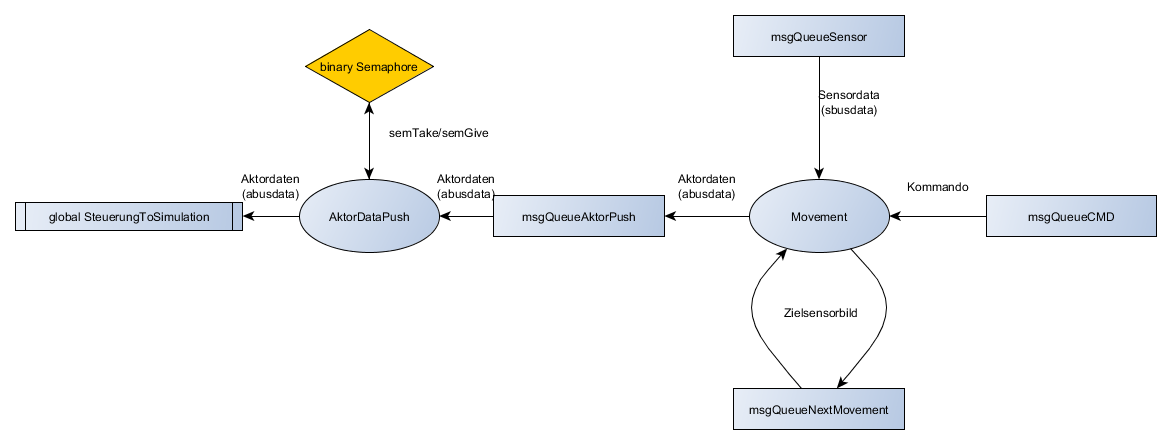
\includegraphics[width=\textwidth]{DFD/dfd1_steuerung.png}
	\caption{DFD1 Steuerung}
	\label{fig3}
\end{figure}

\underline{Mini-Spec Movement:}\\
Der Movement-Task fragt kontinuierlich nach neuem Auftrag aus msgQueueCMD, ist keiner da wird Timeout ausgelöst und System geht in Pause-Modus bzw. Zusatzaufgabe über. Wenn Auftrag bereitsteht wird Belegung geändert(für Befehle vsetspace und clearspace) bzw. es werden die 8 Teilsensorbilder generiert(Befehle insert und remove). Diese werden in msgQueueNextMovement weitergeleitet und werden anschließend nacheinander abgearbeitet (aus der Queue). Für jeden Teilauftrag wird auf neue Sensordaten aus msgQueueSensor gewartet und die daraus entstehenden aktuellen Sensordaten mit den Soll-Sensordaten verglichen, dabei werden alle neuen Sensordaten auf ihre Legitimität überprüft und im Fehlerfall (z.B. blockierte Schiene) werden alle Motoren gestoppt und das System angehalten. Die Aktordoten werden in die msgQueueAktorPush geleitet. \\

\underline{Mini-Spec AktorDataPush:}
AktorDataPush dient zur Weitervermittlung der Aktordaten, welche geschützt weitergeleitet werden müssen(globale Variable).
Wartet auf Aktordaten in msgQueueAktorPush, sind welche vorhanden wartet er auf die Semaphore um anschließend in die globale Variable zu schreiben aus welcher die Simulation liest. Für diese Semaphore wurde eine Prioritätsvererbung implementiert um den Schreibvorgang auf die globale Variable möglichst nicht aus zu bremsen. \\


\subsection {Funktionale Anforderungen}

\paragraph{Beweger}
Wie in Abb.\ref{gantt} zu sehen ist läuft der \textbf{Beweger} als erster Task eines Simulationsschrittes. Zuerst aktualisiert er die Aktorwerte aus der gloablen Variable \textbf{AktorBusData}. Diese entspricht den Busdaten und ist durch eine Semaphore geschützt. Da die Simulation minimal blockiert werden soll implementiert die Semaphore eine Prioritätsvererbung. Daraufhin \glqq verschiebt\grqq   er den virtuellen Turm entsprechend der Aktordaten.

\paragraph{Sensorcollector}
Der \textbf{Sensorcollector} läuft nach allen Sensoren und sammelt  aus einer Message Queue die Einträge aller Sensoren. Wenn ein Sensor ausfällt bleibt der Wert des Sensors auf 1. Daraufhin schiebt er alle Sensorwerte, in einem Vektor, in eine Messega Queue auf die die Steuerung Zugriff hat.

\paragraph{Simulation Sensor x}
Jeder Sensor bekommt eine id übergeben die seine Funktion und ihn eindeutig definiert. 
\begin{enumerate} 
\item \textbf{Tastsensoren} überprüfen ob die Turmposition mit der Sensorposition übereinstimmt.
\item \textbf{Lichtschranken} Simulieren entweder das eintreffen eines Klötzchens am Eingabeslot oder das Entfernen eines Klötzchens am Ausgabeslot, jeweils mit einem vordefinierten Delay.
\item Der \textbf{Lichttaster} im Turm wird dann ausgelöst wenn die vorige y-Position des Turms im vorigen Schritt über (beim Ablegen eines Klötzchens) bzw. unter (beim Aufnehmen) der jetzigen Position ist und (beim Ablegen) ein Klötzchen im Turm ist bzw. (beim Aufnehmen) ein Klötzchen an der Aufnahmeposition ist.
\end{enumerate}
Die jeweiligen Sensordaten schiebt der Task daraufhin in eine Message Queue für den Sensorcollector.

\begin{figure}[H]
	\centering
  \includegraphics[width=\textwidth]{diagrams/gand.png}
	\caption{Gantt Diagramm der Task der Simulation}
	\label{gantt}
\end{figure}

Alle Tasks in der Simulation haben eine Priorität von 200 und ändern diese nicht. Sie werden in einer festen Reihenfolge erzeugt und laufen dann in jedem Zyklus in dieser Sequenz.


\begin{table}[H]
\centering
\begin{tabular}{|l|r|}
\hline
Taster X[0-9] &  [gedrückt|gehalten] \\
\hline
Taster Y[0-9] &  [gedrückt|gehalten] \\
\hline
Taster Z[0-3] &  [gedrückt|gehalten] \\
\hline
Lichtschranke Eingabe & [unterbrochen|nicht unterbrochen] \\
\hline
Lichtschranke Ausgabe & [unterbrochen|nicht unterbrochen] \\
\hline
Turmlichtschalter & [bedeckt|nicht bedeckt]\\
\hline
\end{tabular}
\caption{Requirements Dictionary: Die Stati der Sensoren}
\label{tab:Requirements Dictionary}
\end{table}


\underline{Mini-Spec Sensorcollector:}\\
Der Sensorcollector läuft nach allen Sensoren. Er  greift die Messwerte der einzelnen Sensoren aus \textit{msgQueueIdSensorCollector} ab (leeren der Queue) und fügt sie zu \textit{sbusdata} zusammen und schiebt diese in \textit{msgQueueIdSensorData}.\\ 


\subsubsection{DFD1 Steuerung}
\begin{figure}[H]
	\centering
  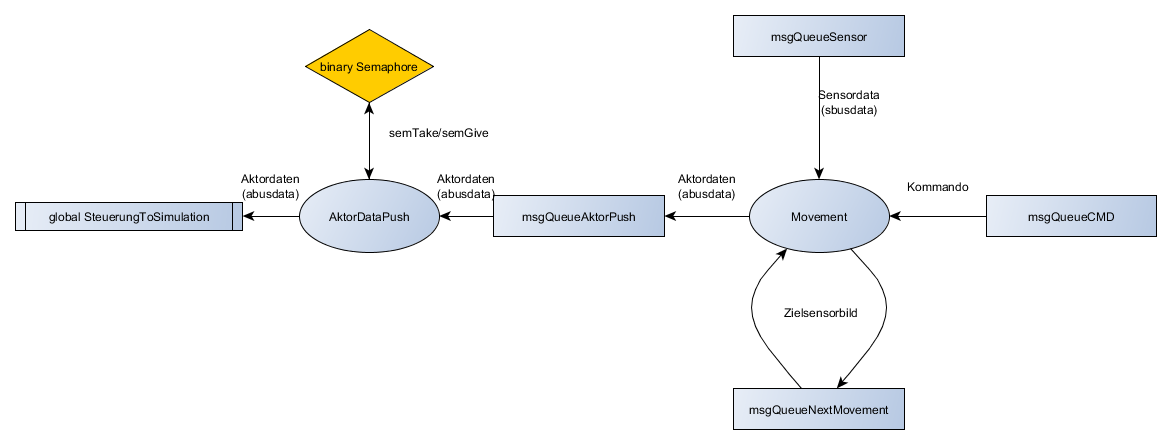
\includegraphics[width=\textwidth]{DFD/dfd1_steuerung.png}
	\caption{DFD1 Steuerung}
	\label{fig3}
\end{figure}

\underline{Mini-Spec Movement:}\\
Der Movement-Task fragt kontinuierlich nach neuem Auftrag aus msgQueueCMD, ist keiner da wird Timeout ausgelöst und System geht in Pause-Modus bzw. Zusatzaufgabe über. Wenn Auftrag bereitsteht wird Belegung geändert(für Befehle vsetspace und clearspace) bzw. es werden die 8 Teilsensorbilder generiert(Befehle insert und remove). Diese werden in msgQueueNextMovement weitergeleitet und werden anschließend nacheinander abgearbeitet (aus der Queue). Für jeden Teilauftrag wird auf neue Sensordaten aus msgQueueSensor gewartet und die daraus entstehenden aktuellen Sensordaten mit den Soll-Sensordaten verglichen und die Aktoren per msgQueueAktorPush angesteuert. \\

\underline{Mini-Spec AktorDataPush:}\\
AktorDataPush dient zur Weitervermittlung der Aktordaten, welche geschützt weitergeleitet werden müssen(globale Variable).
Wartet auf Aktordaten in msgQueueAktorPush, sind welche vorhanden wartet er auf die Semaphore um anschließend in die globale Variable zu schreiben aus welcher die Simulation liest. Für diese Semaphore wurde eine Prioritätsvererbung implementiert um den Schreibvorgang auf die globale Variable möglichst nicht aus zu bremsen. \\